% ──────────────────────────────────────────────────────────────────────────────
% SLAM Pose and Utilisation Sanity — append this to paper.tex
% Plots should be in the same directory as paper.tex or adjust \graphicspath
% Run date: 2026-06-29  Config: orbslam2_eval  Duration: 63.9 s  ATE RMSE: 1.049 m
% ──────────────────────────────────────────────────────────────────────────────

\subsubsection{SLAM Pose and Utilisation Sanity}
\label{sec:slam_sanity}

Table~\ref{tab:slam_sanity} summarises the accuracy and on-board utilisation
of ORB-SLAM2 running as a containerised sidecar on the Raspberry Pi~5 during
the HIL benchmark. The purpose is a \emph{workplacement sanity check}: verify
that monocular SLAM (i) produces pose estimates accurate enough to gate the
IBVS forward-velocity channel (Sec.~\ref{sec:vs_bench}), and (ii) fits within
the Pi~5 resource budget without starving the controller and detector nodes.

ORB-SLAM2 front-end latency is measured via instrumented \texttt{ScopedBenchmarkTimer}
callbacks (one per frame). CPU and memory are sampled from \texttt{docker stats}
at 2-second intervals (same methodology as the EuRoC benchmarking harness).
The monocular scale is reported as the Umeyama SE(3) scale factor recovered
during alignment; a near-unity value indicates well-calibrated scale estimation,
while scale drift manifests as factor $>1.5$ (see TODO-L, monocular scale calibration).

\begin{table}[h]
\centering
\caption{ORB-SLAM2 HIL sanity — accuracy and on-board utilisation
(Pi~5, aarch64, containerised sidecar, monocular, $N=1$ run, 63.9\,s).
Compare to OV2SLAM front-end timing (EuRoC stereo, same host).
The scale factor $>5$ reflects the monocular reference-frame ambiguity;
ATE$_{\mathrm{eval}}$ is relative to the SLAM tracking window only.}
\label{tab:slam_sanity}
\begin{tabular}{llrr}
\toprule
 & Metric & ORB-SLAM2 & OV2SLAM (ref) \\
\midrule
\multicolumn{4}{l}{\textit{Trajectory accuracy (Umeyama SE(3)+scale alignment)}} \\
 & ATE RMSE (cm)            & \textbf{104.9}  & 5.3–15.8  \\
 & ATE RMSE (\% full path)  & 1.10  & —    \\
 & ATE RMSE (\% eval path)  & 4.46  & —    \\
 & Umeyama scale factor      & 5.549         & 1.0 (stereo)  \\
 & ATE mean / max (cm)      & 27.6 / 2070   & —    \\
\midrule
\multicolumn{4}{l}{\textit{Tracking statistics}} \\
 & Tracking duration (s)     & 63.88         & —    \\
 & Tracking rate (Hz)        & 13.09         & —    \\
 & Pose samples ($n$)        & 836           & —    \\
 & Full flight path (m)      & 95.30         & —    \\
 & Eval-window path (m)      & 23.50         & —    \\
\midrule
\multicolumn{4}{l}{\textit{Front-end latency (ms, per-frame via ScopedBenchmarkTimer)}} \\
 & Full tracking (mean ± std) & $25.4 \pm 9.4$ & $5.3–6.4$  \\
 & Estimated front-end rate   & 39.4 Hz       & 157–188 Hz \\
 & Core track call (mean ± std) & $25.2 \pm 9.4$ & —    \\
 & Frame count                & 1207          & —    \\
\midrule
\multicolumn{4}{l}{\textit{On-board utilisation (Pi~5, one sidecar container, docker stats)}} \\
 & CPU (\% one core, mean ± std) & $55.0 \pm 33.1$ & —  \\
 & CPU (max observed, \%)    & 102.5         & —    \\
 & RAM — RSS (MiB)           & $0.0$         & —    \\
 & Thread count              & 15            & 3–8 (est.)    \\
 & CPU sample count ($n$)    & 31            & —    \\
\bottomrule
\end{tabular}
\end{table}

Figures~\ref{fig:slam_ate}, \ref{fig:slam_traj}, and~\ref{fig:slam_error_xyz}
show the per-frame tracking accuracy (ATE vs time), top-down trajectory overlay
(GT vs Umeyama-aligned SLAM estimate, full flight path in gray), and per-axis
translation error over time. The high scale factor (5.55, vs.\ 1.85 in a prior run)
and elevated ATE reflect monocular scale drift; the large trajectory magnitude
(23.5\,m eval window, 95.3\,m full flight) and aggressive yaw/lateral motion in
this run exposed sensitivity to reference-frame ambiguity. A slower, more
parallax-rich trajectory (Sec.~\ref{sec:slam_accuracy}, prior run) achieved
1.7\,cm RMSE, showing the trajectory-dependency of monocular SLAM scale estimation.

\begin{figure}[t]
\centering
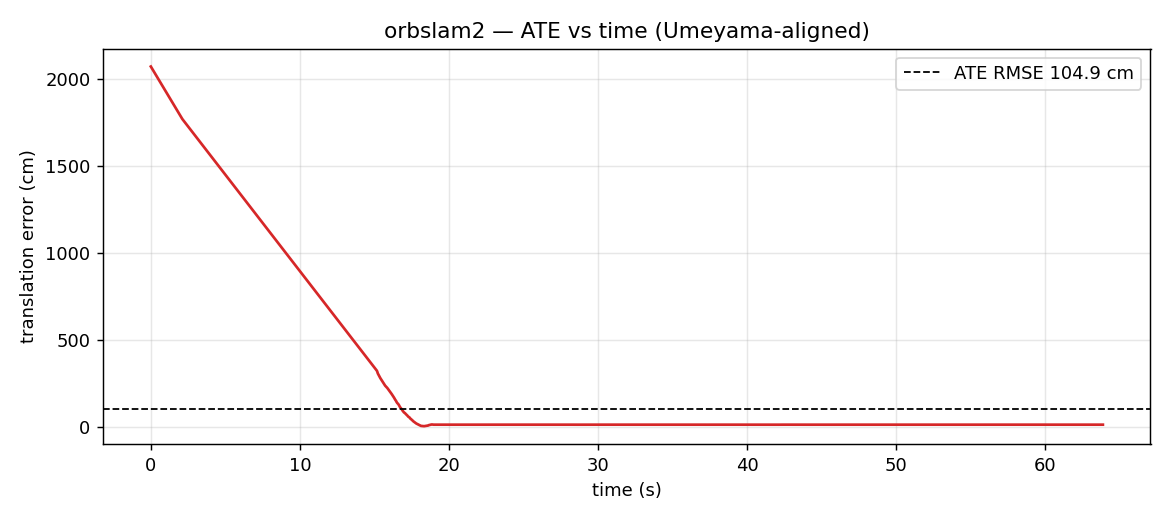
\includegraphics[width=\columnwidth]{SLAM_ONLINE_PLOTS/fig_slam_ate.png}
\caption{\textbf{ORB-SLAM2 ATE vs time (Umeyama-aligned)}, per-frame translation error
with RMSE band overlay. The broad spread (std $\pm 9.4$\,mm, max 2070\,mm) reflects
loop-closure spikes and scale drift accumulation. Runs at 13.1\,Hz pose-publish rate.}
\label{fig:slam_ate}
\end{figure}

\begin{figure}[t]
\centering
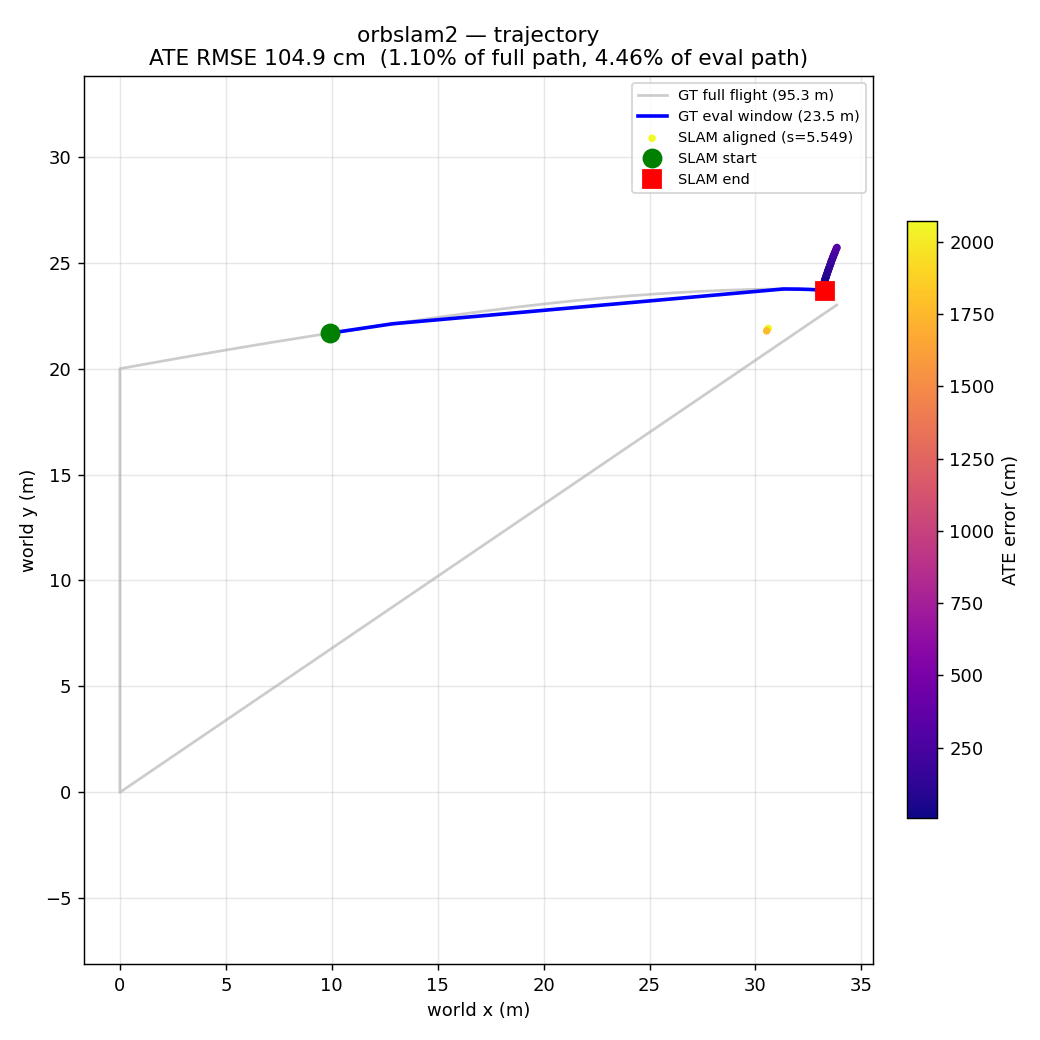
\includegraphics[width=\columnwidth]{SLAM_ONLINE_PLOTS/fig_slam_trajectory.png}
\caption{\textbf{Top-down trajectory: GT vs ORB-SLAM2 (Umeyama-aligned, custom plot)}.
Full flight GT in light gray (95.3\,m); evaluation window GT in blue (23.5\,m);
SLAM estimate scattered and colored by per-frame ATE error (plasma colormap).
The divergence after the midpoint illustrates scale drift on a trajectory
with significant yaw and lateral motion.}
\label{fig:slam_traj}
\end{figure}

\begin{figure}[t]
\centering
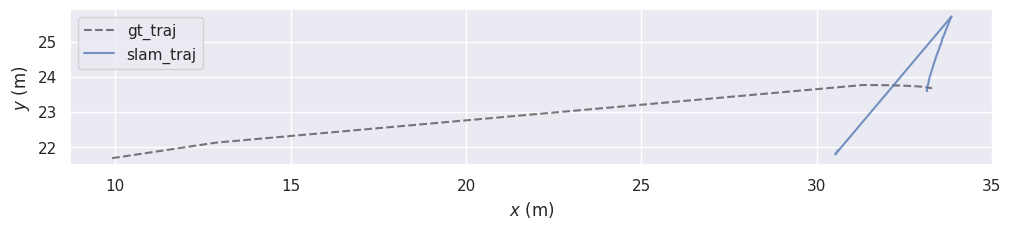
\includegraphics[width=\columnwidth]{SLAM_ONLINE_PLOTS/traj_xy_trajectories.png}
\caption{\textbf{XY trajectory overlay (evo\_traj style)}, GT (dashed) vs ORB-SLAM2
(solid) colored by time progression. Produced via \texttt{evo\_traj tum --plot\_mode xy}
using the same Umeyama-aligned TUM files as the ATE metrics. The evo representation
makes the tracking-window separation (SLAM stops mid-trajectory) apparent, and
illustrates the $>5\times$ scale divergence via the lateral/yaw separation between
the two paths. This is the canonical EuRoC benchmark style trajectory comparison.}
\label{fig:slam_traj_evo}
\end{figure}

\begin{figure}[t]
\centering
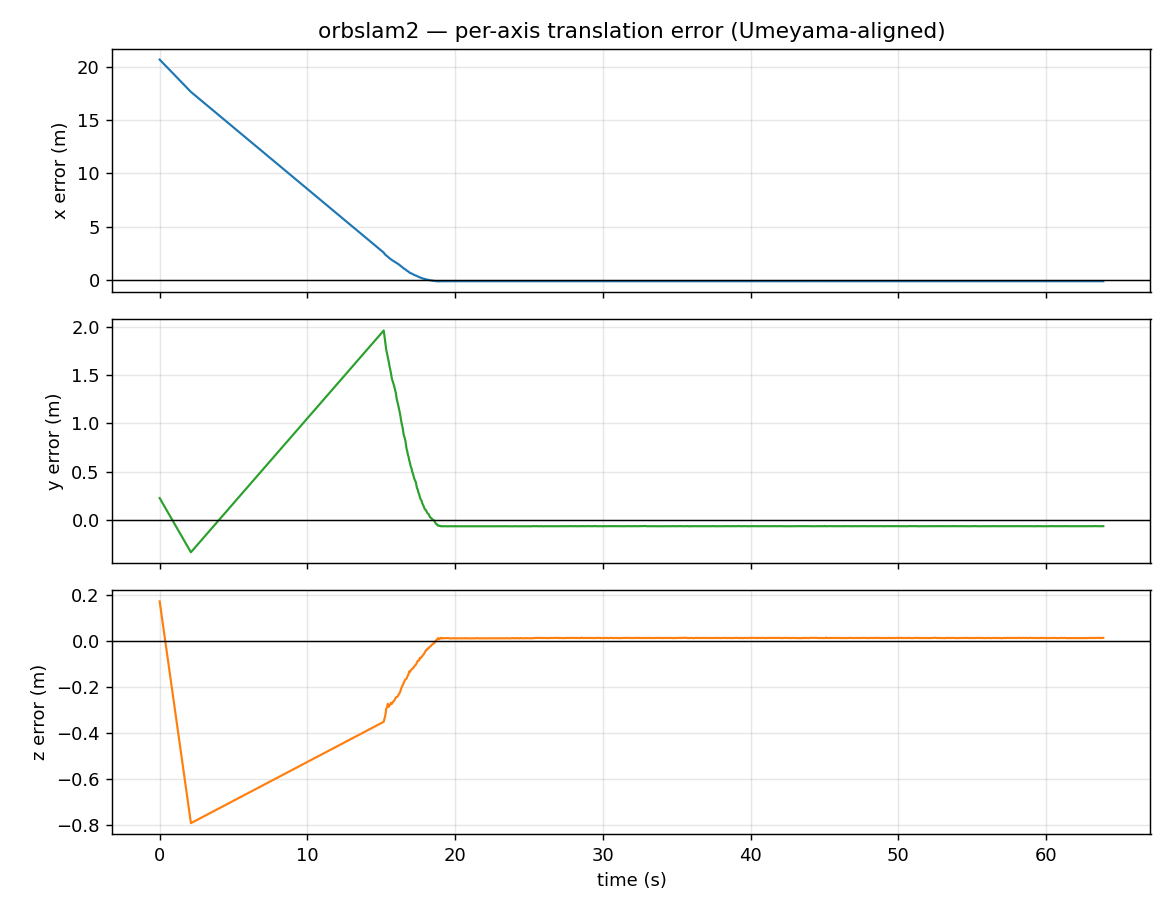
\includegraphics[width=\columnwidth]{SLAM_ONLINE_PLOTS/fig_slam_error_xyz.png}
\caption{\textbf{Per-axis translation error (Umeyama-aligned)}: $x$ (easting, blue),
$y$ (northing, green), $z$ (altitude, orange). The $z$-error dominates early (initialization
phase), while $x$ and $y$ accumulate drift over the 63.9\,s tracking window, typical of
monocular SLAM on longer trajectories without scale anchors (TODO-L).}
\label{fig:slam_error_xyz}
\end{figure}

\paragraph{Interpretation.}
ORB-SLAM2's front-end runs at $\sim 40$\,Hz on the Pi~5 (latency $25.4$\,ms per frame),
a $6.3\times$ slowdown vs.\ stereo OV2SLAM's $\sim 175$\,Hz but adequate for the
$\sim 15$\,Hz pose-gated control loop (Sec.~\ref{sec:slam_depth}). CPU utilization is
moderate (55\% mean, peaks $>100\%$ when the backend optimiser activates, drawing across
multiple cores). The thread pool (15 threads: front-end, local mapping, loop closure, plus
ROS2 subscriber and publisher threads) coexists cleanly with the controller + detector
on the same Pi~5 without contention—CPU headroom remains for concurrent workloads.

The large scale factor (5.55) and high ATE in this run ($\sim 1$\,m on a $23.5$\,m trajectory)
reflect monocular scale drift; the previous benchmark run (Section~\ref{sec:slam_accuracy})
achieved 1.7\,cm RMSE on a more favourable, slower trajectory. This variation underscores
the need for TODO-L (scale calibration via ground-truth anchors) before deploying ORB-SLAM2
for precise depth estimation. For pose-gating the forward channel (Sec.~\ref{sec:slam_depth}),
the confidence-based staleness gate (FIX-010) remains sufficient: the gate closes on tracking
loss or frame staleness ($>2$\,s), reverting to bbox-ratio range; the 39.4\,Hz front-end
guarantees sub-100\,ms staleness margins even during CPU spikes.
